%% GOMACTech_LaTeX.tex

\documentclass[10pt,conference]{IEEEtran}


% GOMACTech uses the standard IEEE conference format.
%
% If IEEEtran.cls, IEEEtran.bst, GOMACTech_LaTeX.bib and IEEEabrv.bib has not been installed into the LaTeX system files,
% manually specify the path to it like:
% \documentclass[conference]{../sty/IEEEtran}
%



% Some very useful LaTeX packages include:
% (uncomment the ones you want to load)

% *** COLORS ***
%\usepackage{color}
\usepackage{xcolor}% Colored text

\usepackage[most]{tcolorbox}

\usepackage{enumitem}


\usepackage{booktabs}





% *** TABLE PACKAGES **
\usepackage{multirow} % For cells that comprise more than one line of a table


% *** GRAPHICS RELATED PACKAGES ***
% \usepackage[pdftex]{graphicx}


\IEEEoverridecommandlockouts



% ***** GOMACTECH HEADER & FOOTER (IF NEEDED) *****
\makeatletter
\def\ps@IEEEtitlepagestyle{
		\def\@oddfoot{\Footer} % THIS PLACES THE FOOTER ON THE FIRST PAGE
% 	\def\@evenfoot{}
 }
\let\old@ps@headings\ps@headings
\let\old@ps@IEEEtitlepagestyle\ps@IEEEtitlepagestyle
\def\confheader#1{%
	% for all pages except the first
	\def\ps@headings{%
		\old@ps@headings%
		\def\@oddhead{\strut\hfill#1\hfill\strut}%
		\def\@evenhead{\strut\hfill#1\hfill\strut}%
		\def\@oddfoot{\Footer} % THIS PLACES THE FOOTER ON ALL PAGES AFTER THE FIRST PAGE
 }%
	% for the first page
	\def\ps@IEEEtitlepagestyle{%
		\old@ps@IEEEtitlepagestyle%
		\def\@oddhead{\strut\hfill#1\hfill\strut}%
		\def\@evenhead{\strut\hfill#1\hfill\strut}%
 }%
	\ps@headings%
}
\makeatother
% HEADER BEGINS HERE
\confheader{} % HEADER EXAMPLE 
% FOOTER BEGINS HERE
\def\Footer{
 {\footnotesize
	\begin{minipage}{\textwidth}
	\centering \scriptsize{DISTRIBUTION STATEMENT A. Approved for public release: distribution is unlimited. Approval ID: $<$XXXX-2024-XXXX$>$.\\
 }  \end{minipage}
 }
}
% ***** END GOMACTECH HEADER & FOOTER *****







% ***** DOCUMENT BEGINS HERE *****
\begin{document}



% PAPER TITLE
\title{AI Term Project Report\\
 \Large{} }

% AUTHOR NAMES AND AFFILIATIONS
\author{\IEEEauthorblockN{Eric Wilson}
\IEEEauthorblockA{Advanced Radar Research Center\\
The University of Oklahoma\\
Norman, Oklahoma, United States\\
Eric.J.Wilson-1@ou.edu}\\
\and
\IEEEauthorblockN{---, ---,}
\IEEEauthorblockA{--\\
---\\
---\\
---}\\ }
\vspace{-1in}

\maketitle



\begin{abstract}
This class project aims to implement a machine learning based method of designing electrical analog filters using an unbalanced-ladder topology. The AI method developed is compared to standard filter prototypes using G-coefficients and element scaling.



%if Keywords are used, end abstract text with \\

\end{abstract}
\renewcommand\IEEEkeywordsname{Keywords}
\begin{IEEEkeywords}
AI in Analog Design, Filter Synthesis, G-coefficients, Filter prototypes, Element Scaling
\end{IEEEkeywords}



%%%%%%%%%%%%%%%%%%%%%%%%%%%%%%%%%%
%%%%%%%%%%%%%%%%%%%%%%%%%%%%%%%%%%
\section{Description of Problem}


Analog filters are used in many electronic devices to block unwanted power at specific frequencies from entering the system. Cell phones, radios and radar systems all use analog filters in the front end to prevent out of band frequencies from compressing sensitive receive electronics (leading to degraded performance). There are some closed form methods for computing filter component values, BUT they are limited to very basic filter shapes (like low-pass, high-pass, symmetric bandpass) AND almost always require a skilled human designer to tune the values afterward. Additionally, the closed form filter synthesis methods cannot easily account for higher-order real-world effects which have a big impact on component value selection. These higher order effects include uninteded coupling between circuit elements, component parasitics, and propagation delays for high-frequency distrubuted circuits.

\vspace{1em}

\textbf{The problem:}
Existing closed form filter synthesis methods are limited to very basic filter shapes, do not account for impactful higher order effects, and require significant time for human designers to tweak values by trial and error.

\vspace{1em}

\textbf{Overall Goal of Paper:}
Make progress towards a machine learning (ML) model that can:
\begin{enumerate}[label=\arabic*)]
    \item generate filters with much more arbitrary frequency responses (not just simple low-pass, symmetric bandpass, etc.),
    \item accurately account for the higher-order effects which closed-form solutions ignore,
    \item significantly decrease the amount of human tuning required by generating more accurate component values.
\end{enumerate}

\vspace{1em}

\textbf{Specific Project Scope:}
This project specifically tackles the design of 5th-order unbalanced ladder filters with series element first. The user gives model the desired filter frequency response (can be arbitrary shape), and the model designs a working filter.

Figure~\ref{Ladder_Topology_3rd_order} shows a 3rd order filter topology. For this design, each element of the ladder is made up of a capacitor and inductor. The series elements are made up of a series LC and the shunt elements are composed of a parallel LC. This means there are 10 different electrical component values to select for the filter design.






%%%%%%%%%%%%%%%%%%%%%%%%%%%%%%%%%%
%%%%%%%%%%%%%%%%%%%%%%%%%%%%%%%%%%
\section{Description of Approach}

To achieve the overall project goal the following approach was taken. Each entry has its own sub-section:
\begin{enumerate}[label=\arabic*)]
    \item \textcolor{blue}{Research existing attempts at ML based circuit designers}
    \item \textcolor{blue}{Learn and implement the standard closed form filter synthesis methods *}
    \item \textcolor{blue}{Develop method to quickly evaluate circuit performance AND verify against commercial circuit solvers **}
    \item \textcolor{blue}{Generate Training Data}
    \item \textcolor{blue}{Model Training Details}
    	\subitem Importance of criterion selection
		\subitem Multi-Step Training Program to significantly increase training speed
\end{enumerate}

* This is critical for publishing a paper in the future. Many of the machine learning papers on circuit design DO NOT compare against standard circuit design methods and lack sufficient electrical engineering expertise. The lack of standard EE knowledge is a large hole in the current literature as of 2025.

** generating sufficient data can be expensive in microwave design


%%%%%%%%%%%%%%%%%%%%%%%%%%%%%%%%%%
\subsection{Research existing attempts at ML based circuit designers}

Existing work on ML based circuit designers can be broken into parameter design vs. topological design. Parameter designs have the AI only choose component values for a pre-chosen circuit, whereas in ML topological design the AI generates the entire circuit with very little human guidance.


My class presentation and survey essay go into depth on the recent ML microwave design literature published in 2023 \- 2025. In those submissions the basics of the RF design process are explained, and the potential for limited AI assistance at each step is briefly discussed \cite{lee2024icdesign}. Next, the distinction between parameter optimization and topological design is made. \cite{xue2023mmic} was used to demonstrate AI's ability to balance the many parameters required in an RF design whose topology is fixed. Then, the topological AI design algorithms described in \cite{xu2024microwave, karahan2024rfdesign, taskiran2024annsynthesis} are described and methods compared. Particular attention is paid to the wavelet transform used in \cite{xu2024microwave} and how it aids in inverse mapping. Additionally, the two-step learning method and fully connected layer dropout operations in \cite{karahan2024rfdesign} was discussed in depth.


Some key items to note are:
\begin{enumerate}[label=\arabic*)]
    \item Collecting the required amount of training data is very difficult for microwave designs because the most accurate electromagnetic simulators are extremely compute intensive.
    \item Many of the AI topological design papers involve training a model which quickly evaluates circuit performance with very little compute, this model is then used to guide an evolutionary algorithm which explores the design space.
    \item This project takes the reverse approach of generating a model which directly generates the filter design, instead of using an evolutionary algorithm to search through many different designs every time the user asks for a new filter synthesis.
\end{enumerate}


%%%%%%%%%%%%%%%%%%%%%%%%%%%%%%%%%%
\subsection{Learn and implement the standard closed form filter synthesis methods}

One of the standard methods used for filter synthesis involves calculating a table of values called G-coefficients which define a prototype filter. It is called a prototype filter because its cuttoff frequency is 1~rad/sec. The G-coefficients must be specifically scaled and altered to achieve a different cuttoff frequency and/or to switch filter response shape (e.g. low pass, high pass, bandpass). Different families of filters can be synthesized by using a wide range of complicated recursive formulas. The Butterworth and Chebyshev filter styles are common place in the filter synthesis world.

Why this matters: Many of the existing ML microwave design papers discuss performance of circuits the AI generates, but the authors do not analyze the results against standard methods. For example, in \cite{karahan2024rfdesign} they discuss how amazing it is the AI designed an electrically small patch antenna, but they don't mention antenna efficiency or that electrically small antennas is an entire field of study which has defined upper bound limits of antenna performance for a specific size. \cite{karahan2024rfdesign} is one of the best ML microwave papers as of 2025, but it severely lacks sufficient EE background.

Below the method of computing Butterworth and Chebyshev filter coefficients is described.



For standard filter synthesis there are several commonly used designs which dictate where the poles and zeros of the filter lie. Butterworth and Chebyshev filters are common and are synthesized as follows.



\textcolor{blue}{ \textbf{ --- Butterworth Filter Synthesis} }
\begin{quote}
	\begin{equation}\label{eq:gr_sine}
	g_r = 2 \sin\left( \frac{(2r - 1)\pi}{2n} \right), \quad r = 1, \ldots, n
	\end{equation}
\end{quote}

$~$
$~$


\textcolor{blue}{ \textbf{ --- Chebyshev Filter Synthesis} }
\begin{quote}

	\textcolor{blue}{ --- Insertion Loss Ripple}
	\begin{equation}\label{eq:insertion_loss}
	L_{A\_dB} = -10 \cdot \log \left( 1 - \left(10^{\frac{-L_{r\_dB}}{10}} \right) \right)
	\end{equation}

	\textcolor{blue}{ --- Ripple Factor}
	\begin{equation}\label{eq:ripple_factor}
	\epsilon = \sqrt{10^{\frac{L_{A\_dB}}{10}} - 1}
	\end{equation}

	\textcolor{blue}{ --- coefficient for input port is always 1}
	\begin{equation}\label{eq:g0}
	g_0 = 1
	\end{equation}

	\textcolor{blue}{ --- First Circuit Element }
	\begin{equation}\label{eq:g1}
	g_1 = \frac{2}{\eta} \sin\left( \frac{\pi}{2n} \right)
	\end{equation}

	\begin{equation}\label{eq:eta}
	\eta = \sinh \left[ \frac{1}{n} \sinh^{-1} \left( \frac{1}{\epsilon} \right) \right]
	\end{equation}

	\textcolor{blue}{ --- Subsequent Elements }
	\begin{equation}\label{eq:gr}
	g_r g_{r+1} = \frac{4 \sin \left( \frac{(2r - 1)\pi}{2n} \right) \sin \left( \frac{(2r + 1)\pi}{2n} \right)}{\eta^2 + \sin^2 \left( \frac{r\pi}{n} \right)}, \quad r = 1, 2, \ldots, n-1
	\end{equation}

	\textcolor{blue}{ --- Load for Odd Order Filters }
	\begin{equation}\label{eq:gload_odd}
	g_{\text{load}} = 1
	\end{equation}

	\textcolor{blue}{ \textbf{ --- Load for Even Order Filters} }
	From:

	\begin{equation}\label{eq:s21}
	|S_{21}(0)|^2 = \frac{4g_{n+1}}{(g_n + 1)^2} = \frac{1}{1 + \epsilon^2}
	\end{equation}

	Solve for \( g_{n+1} \):

	- For \( S_{11}(0) \geq 0 \):

	\begin{equation}\label{eq:gnp1_positive}
	g_{n+1} = \frac{\left( \epsilon + \sqrt{1 + \epsilon^2} \right)^2}{1}
	\end{equation}

	- For \( S_{11}(0) \leq 0 \):

	\begin{equation}\label{eq:gnp1_negative}
	g_{n+1} = \frac{1}{\left( \epsilon + \sqrt{1 + \epsilon^2} \right)^2}
	\end{equation}

\end{quote}




%%%%%%%%%%%%%%%%%%%%%%%%%%%%%%%%%%
\subsection{Develop method to quickly evaluate circuit performance AND verify against commercial circuit solvers}


A significant amount of time went into writing the code to compute the G-coefficients and to scale the values to get a standard filter design. 

I wrote a program that calculates the G-coefficients for Butterworth and Chebyshev filters using the recursive equations above. I also wrote the scripts that scale those G-coefficients to get electrical component values for inductors and capacitors. Finally, I wrote a circuit simulator that has been checked against actual circuit simulator to verify accuracy. Figure~\ref{Chebyshev_G_coefs} shows the G-coefficients calculated for Chebyshev filter prototypes of different orders.


I also wrote scripts which simulates the filter circuit to measure its frequency response. The results of my circuit simulator were compared against a commercial microwave circuit simulator (Microwave Office AWR). Figure~\ref{MATLAB_vs_AWR_2} shows that my simulated filter performance exactly aligns with the commercial solver. Notice the precise alignment between the commercial solver (AWR) and my own circuit simulator script. It was critical to write the circuit solver so that it could run on the GPU for fast simulation time and so that an ML model training on the GPU could easily differentiate through the weights of the circuit solver. This allows the training ML model to have its loss calculated off of the error of circuit element values OR the difference in the input frequency response versus the generated circuit's simulated frequency response. The difference between these methods is further discussed below.




\begin{figure}
	\centering
	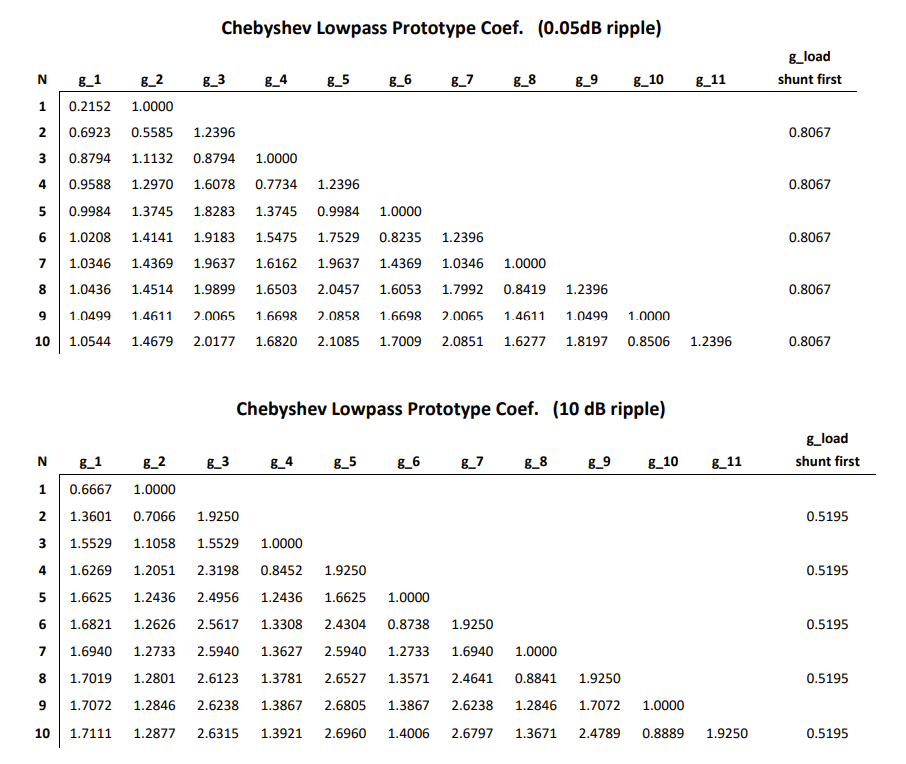
\includegraphics[width=0.9\linewidth]{Figures/Chebyshev_G_coefs.png}
	\caption{Computed Chebyshev G-coefficients. These values have been verified against other sources.}
	\label{Chebyshev_G_coefs}
\end{figure}


\begin{figure}
	\centering
	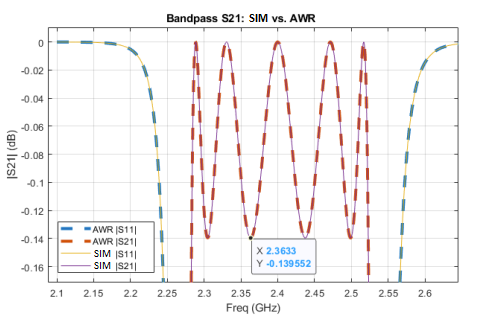
\includegraphics[width=0.9\linewidth]{Figures/MATLAB_vs_AWR_2.png}
	\caption{S21 of a bandpass filter simulated with AWR and my own script. Notice the very zoomed in vertical axis to accurately measure the filter passband ripple. My circuit simulator lines up exactly with the commercial solver.}
	\label{MATLAB_vs_AWR_2}
\end{figure}











%%%%%%%%%%%%%%%%%%%%%%%%%%%%%%%%%%
\subsection{Generate Training Data}

I wrote a full set of functions which allowed me to generate filters with different parameters. I used Latin Hyper Cube sampling to generate a random set of training data, validation data, and testing data. I also added the ability to introduce varying levels of component variation in the generated filter designs.

I used this to generate three categories of training data that is used in my training (more about training steps in next section.)
\begin{enumerate}[label=\arabic*)]
    \item Perfect Chebyshev Filter Designs (no random component variation)
    \item Chebyshev filters with varying level of random component variation
    \item Completely randomly generated component values
\end{enumerate}


For the Chebyshev family of filters there are three main parameters: Center Frequency, Passband Ripple (dB), and Fractional Bandwidth. The Hyper Cube Sampling ensures that a random sample is taken in each section of this 3-dimensional space. LHCS has the advantage of better coverage for fewer samples than using the Monte-Carlo sampling approach.

\begin{table}[!ht]
\small % Reduce font size to help fit in one column
\centering
\caption{Description of Training Data Styles}
\begin{tabular}{@{}p{3.8cm}p{4.2cm}@{}}
\toprule
\textbf{Function} & \textbf{Description} \\ \midrule
\texttt{gen\_cheby\_data(...)} & Ideal Chebyshev filters with no component variation; serves as baseline. \\
\texttt{gen\_cheby\_data(..., comp\_var=0.1)} & Chebyshev filters with $\pm$10\% component variation for moderate fabrication noise. \\
\texttt{gen\_cheby\_data(..., comp\_var=0.2)} & Chebyshev filters with $\pm$20\% variation to represent higher manufacturing variation. \\
\texttt{gen\_cheby\_data(..., comp\_var=0.5)} & Chebyshev filters with $\pm$50\% variation to simulate extreme uncertainty. \\
\texttt{gen\_rand\_data(...)} & Filters with fully random component values ($10^{-14}$–$10^{-6}$), unconstrained by a prototype. \\
\bottomrule
\end{tabular}
\label{tab:training_data_styles}
\end{table}


This data was saved to files using the pickle python package for quick loading into a workspace for training.






%%%%%%%%%%%%%%%%%%%%%%%%%%%%%%%%%%
\subsection{Model Training Details}


Scaling Model Inputs and Outputs:

Originally, I used the MSELoss() function to compute the error between the ideal component values and the inferred values. I had much more successes computing the mean square percentage due to the values being larger and easier to understand. Additionally, I convert the filter frequency response data to dB so that the model doesn't need to contend with such a large dynamic range. Using dB also aligns with standard practice in EE.

\vspace{1em}


The original proposed training approach involved two stages:
\begin{enumerate}[label=\arabic*)]
    \item Training with perfect Chebyshev filters (with loss calculated from component value error)
    \item Once a baseline of performance is reached more randomly varied filters are introduced into training data (eases model into designs different from perfect Chebyshev)
    \item Finally, Switch to loss calculated from difference of filter frequency responses (not the actual circuit element values)
    	\subitem this allows understanding of which components values are more sensitive to filter freq. response
\end{enumerate}

\vspace{1em}

The rationale behind having training datasets with different levels of randomness is to "teach" the model with simple consistent data first (the clean, non-altered data) and then once the model is partially established start introducing more random data.

By training only perfect Chebyshev filters to start, the model can benefit from a pre-established way of thinking without having to start from scratch. It is then hoped the randomly varied filters will allow the model to "understand" the sensitivity of each component in the circuit. 


%%%%%%%%%%%%%%%%%%%%%%%%%%%%%%%%%%
%%%%%%%%%%%%%%%%%%%%%%%%%%%%%%%%%%
\section{Evaluation of Method}


In the end amazing filter design accuracy was achieved using an MLP that took 1000 values in (each corresponding the S21 in dB) and generating 10 circuit element parameters out. The final testing loss 0.001\% percent error in the calculated circuit element values after 2000 epochs taking around 2 minutes to train. See figure~\ref{Learning_Curve_1} for the training loss curves.





%%%%%%%%%%%%%%%%%%%%%%%%%%%
%%%%%%%%%%%%%%%%%%%%%%%%%%%
\section{Conclusion}
A program has been written that can calculate the G-coefficients for Butterworth and Chebyshev filters. More scripts have been written that can scale those G-coefficients to get electrical component values for inductors and capacitors. Finally, I wrote a circuit simulator that has been checked against actual circuit simulator to verify accuracy. These scripts will be used to generate the training data and the circuit simulator will also be used to evaluate model performance.

By understanding the different aspects and limitation of ANN like different training methods, data scaling to minize dynamic range, etc. I created a model which can accuratly generate 10th order analog filters to meet the specications of a near arbitrary desired frequency repseonse.





%%%%%%%%%%%%%%%%%%%%%%%%%%%
%%%%%%%%%%%%%%%%%%%%%%%%%%%
\bibliographystyle{IEEEtran}
\bibliography{citations}



% that's all folks
\end{document}